\documentclass[10pt,openright,twoside,french]{book}

\input philippe2013
\input philippe2013_cours
\input philippe2013_sections
\input philippe2013_chapitre


\begin{document}
\setcounter{chapter}{2}
\renewcommand\PartProgramme{Fonctions}
\chapter[Généralités sur les fonctions]{Généralités sur\\ les fonctions}\label{ch_gen_fonctions}

\section{Notions}

\begin{Defi}
    Soit $\calig D_f$ un ensemble de nombres réels (généralement un intervalle ou une réunion d'intervalles).
    Définir une \ipt{fonction} $f$ sur $\calig D_f$, c'est associer à tout nombre $x$ de $\calig D_f$ un réel unique, noté $f(x)$ et appelé \ipt{image} de $x$ par $f$.\par
    $x$ est appelée la \ipt{variable} et $f(x)$ est la valeur prise par la fonction $f$ pour la valeur $x$.\par
    L'ensemble $\calig D_f$ est appelé \ipt{ensemble de définition} de $f$ (ou domaine de définition).
\end{Defi}\medskip

\textbf{Notation :}\quad La phrase : \textit{\og~La fonction $f$ qui, au nombre $x$, associe le nombre $f(x)$~\fg}\par
\textcolor{white}{\textbf{Notation }\quad} peut se noter de la façon suivante : $f : x \mapsto f(x)$.\medskip

\begin{Exemple}[s]
    \begin{enumerate}
        \item Soit $g$ la fonction qui, à $x$, associe le nombre $2x^2 - 1$.\par Elle est définie par $g(x) = 2x^2 -1$ et on note : $g : x \mapsto 2x^2 - 1.$
        \item Si on considère la taille associée à un individu, on définit une fonction : \textit{individu} $\mapsto$ \textit{taille}.
        \item	Si on considère le prix de vente d'un litre d'essence dans une ville, on ne définit pas une fonction car pour un même type d'essence, il peut exister plusieurs prix en fonction des stations service.
    \end{enumerate}
\end{Exemple}\medskip

Pour avoir une idée visuelle de la fonction, il est souvent utile de la représenter graphiquement dans un repère orthonormé. On a alors la définition suivante :\medskip

\begin{Defi}
Soit $f$ une fonction définie sur $\calig D_f$.\par
Dans un repère du plan, la \ipt{courbe représentative} $\calig C_f$ de $f$ est l'ensemble des points $M$ de coordonnées $(x_M \pv y_M)$ telles que :
\begin{itemize}
    \item $x_M$ décrit l'ensemble de définition $\calig D_f$ ;
    \item $y_M$ est l'image de $x_M$ par $f$ : $y_M = f(x_M)$.
\end{itemize}
\end{Defi}\medskip

\begin{Rmq}
    On dit que $\calig C_f$ a pour équation $y = f(x)$ dans le repère choisi.
\end{Rmq}\medskip

\begin{center}
    \begin{tikzpicture}[scale=1.2]
        \draw[->,blue] (-1.75,0)--(4,0);
        \draw[->,blue] (0,-0.25)--(0,3);
        \draw[color=red,line width=1pt] plot[domain=-1.25:3.6,samples=200] (\x,{cos(deg(\x))+1.5});
        \coordinate (M) at (1.5,{cos(deg(1.5))+1.5}); \draw (M) node{\large $+$};
        \draw[dashed] (1.5,0)|-(0,{cos(deg(1.5))+1.5});
        \begin{scriptsize}
            \draw (M) node[above right]{$M$};
            \draw (1.5,0) node[below] {$x_M$};
            \draw (0,{cos(deg(1.5))+1.5}) node[left] {$y_M=f(x_M)$};
            \draw (3.5,{cos(deg(3.5))+1.5}) node[above] {$\calig C_f$};
        \end{scriptsize}
    \end{tikzpicture}
\end{center}\clearpage

\begin{Defi}
    On considère une fonction $f : x \mapsto f(x)$.\par
    Soit $y$ un nombre réel pour lequel il existe $x \in \calig D_f$ tel que $y = f(x)$.\par
    On dit alors que $x$ est un \ipt{antécédent} de $y$ par $f$.
\end{Defi}

\begin{Rmq}
    D'après les définitions précédentes, on en déduit que l'image d'un nombre de $\calig D_f$ existe toujours et est \textbf{unique} alors qu'un nombre peut avoir plusieurs antécédents (voire aucun).
\end{Rmq}

\section{Définir une fonction}
\subsection{À partir d'une courbe représentative}

\begin{tabularx}{\linewidth}{|X|X|X|}
\hline
\textbf{Ensemble de définition} & \textbf{Lecture d'image} & \textbf{Lecture d'antécédents} \\
\hline
%-- colonne 1
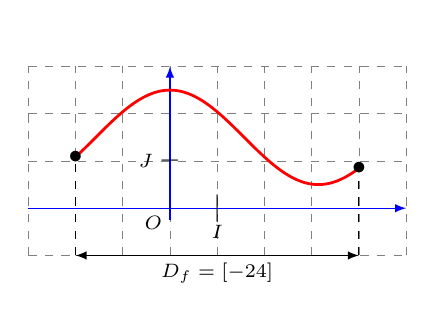
\begin{tikzpicture}[scale=0.6,>=latex]
    \draw[dashed,very thin,color = gray] (-3,-1) grid (5,3);
    \draw[->,blue] (-3,0)--(5,0);
    \draw[->,blue] (0,-0.25)--(0,3);
    \draw[color=red,line width=1pt] plot[domain=-2:4,samples=200] (\x,{cos(deg(\x))+1.5});
    \draw[dashed] (-2,-1)--(-2,{cos(deg(-2))+1.5});
    \draw[dashed] (4,-1)--(4,{cos(deg(4))+1.5});
    \draw (-2,{cos(deg(-2))+1.5}) node{\rouge{$ \bullet$}};
    \draw (4,{cos(deg(4))+1.5}) node{\rouge{$ \bullet$}};
    \draw (1,0) node {$|$};\draw (0,1) node {$-$};
    \draw (0,3.5) node {\textcolor{white}{a}};
    \begin{scriptsize}
        \draw[<->] (-2,-1)--(4,-1) node[midway,below] {$\calig D_f = [-2 \pv 4]$};
        \draw (0,0) node[below left]{$O$};
        \draw (1,-0.2) node[below]{$I$};
        \draw (-0.2,1) node[left]{$J$};
    \end{scriptsize}
\end{tikzpicture}&
%-- colonne 2
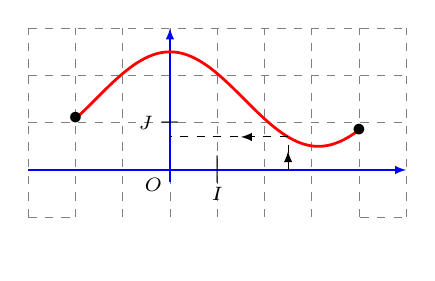
\begin{tikzpicture}[scale=0.6,>=latex]
    \draw[dashed,very thin,color = gray] (-3,-1) grid (5,3);
    \draw[->,blue] (-3,0)--(5,0);
    \draw[->,blue] (0,-0.25)--(0,3);
    \draw[color=red,line width=1pt] plot[domain=-2:4,samples=200] (\x,{cos(deg(\x))+1.5});
    \draw (-2,{cos(deg(-2))+1.5}) node{\rouge{$ \bullet$}};
    \draw (4,{cos(deg(4))+1.5}) node{\rouge{$ \bullet$}};
    \draw (1,0) node {$|$};\draw (0,1) node {$-$};
    \draw[dashed] (2.5,0)|-(0,{cos(deg(2.5))+1.5});
    \draw[->](2.5,0.3)--(2.5,0.4);
    \draw[->](1.6,{cos(deg(2.5))+1.5})--(1.5,{cos(deg(2.5))+1.5});
    \begin{scriptsize}
        \draw (0,0) node[below left]{$O$};
        \draw (1,-0.2) node[below]{$I$};
        \draw (-0.2,1) node[left]{$J$};
        \draw[white] (-2,-1)--(4,-1) node[midway,below] {\textcolor{white}{$\calig D_f = [-2 \pv 4]$}};
    \end{scriptsize}
\end{tikzpicture}&
%-- colonne 3
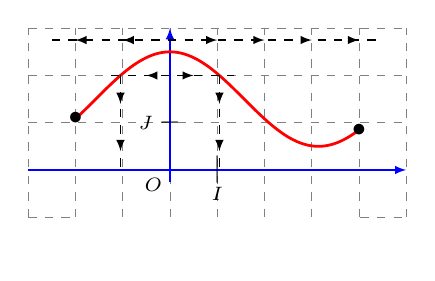
\begin{tikzpicture}[scale=0.6,>=latex]
    \draw[dashed,very thin,color = gray] (-3,-1) grid (5,3);
    \draw[->,blue] (-3,0)--(5,0);
    \draw[->,blue] (0,-0.25)--(0,3);
    \draw[color=red,line width=1pt] plot[domain=-2:4,samples=200] (\x,{cos(deg(\x))+1.5});
    \draw (-2,{cos(deg(-2))+1.5}) node{\rouge{$ \bullet$}};
    \draw (4,{cos(deg(4))+1.5}) node{\rouge{$ \bullet$}};
    \draw (1,0) node {$|$};\draw (0,1) node {$-$};
    \draw[dashed] (-2.5,2.75)--(4.5,2.75);
    \draw[dashed] ({acos((0.5))*pi/180},2)--({acos((0.5))*pi/180},0);
    \draw[dashed] ({-acos((0.5))*pi/180},2)--({-acos((0.5))*pi/180},0);
    \draw[dashed] ({-acos((0.5))*pi/180-0.2},2)--({acos((0.5))*pi/180+0.3},2);
    \draw[->](-0.4,2)--(-0.5,2);
    \draw[->](0.4,2)--(0.5,2);
    %
    \draw[->] ({acos((0.5))*pi/180},1.5)--({acos((0.5))*pi/180},1.4);
    \draw[->] ({-acos((0.5))*pi/180},1.5)--({-acos((0.5))*pi/180},1.4);
    \draw[->] ({acos((0.5))*pi/180},0.5)--({acos((0.5))*pi/180},0.4);
    \draw[->] ({-acos((0.5))*pi/180},0.5)--({-acos((0.5))*pi/180},0.4);
    %
    \draw[->] (-0.9,2.75)--(-1,2.75);
    \draw[->] (0.9,2.75)--(1,2.75);
    \draw[->] (-1.9,2.75)--(-2,2.75);
    \draw[->] (1.9,2.75)--(2,2.75);
    \draw[->] (2.9,2.75)--(3,2.75);
    \draw[->] (3.9,2.75)--(4,2.75);
    \begin{scriptsize}
        \draw (0,0) node[below left]{$O$};
        \draw (1,-0.2) node[below]{$I$};
        \draw (-0.2,1) node[left]{$J$};
        \draw[white] (-2,-1)--(4,-1) node[midway,below] {\textcolor{white}{$\calig D_f = [-2 \pv 4]$}};
    \end{scriptsize}
\end{tikzpicture} \\
\hline
Lecture de l'ensemble de définition sur l'axe des abscisses. &
Image d'un nombre sur l'axe des ordonnées. Ici, l'image de $2,5$ est environ $0,8$. &
Lecture d'antécédents sur l'axe des abscisses. Ici, $2$ a pour antécédent environ $-1$ et $1$. $2,75$ n'a pas d'antécédent.\\
\hline
\end{tabularx}\bigskip

\subsection{À partir d'un tableau}
On considère la fonction $f$ définie de la façon suivante :

\begin{center}
\begin{tabular}{|*{6}{c|}}
\hline
$x$ & $-2$ & $-1$ & $0$ & $1$ & $2$ \\
\hline
$f(x)$ & $1$ & $3$ & $8$ & $10$ & $3$ \\
\hline
\end{tabular}
\end{center}\bigskip

\begin{description}
    \item[Ensemble de définition.] La fonction n'est définie que pour les valeurs de $x$ écrites sur la première ligne du tableau. En dehors de ces nombres, on ne sait pas ce qu'il se passe.
    \item[Lecture d'image.] On sait que l'image de $x$ est $f(x)$ : on lit l'image d'un nombre de la première ligne dans la deuxième ligne. Par exemple, $f(1) = 10$.
    \item[Lecture d'antécédents.] Les antécédents se lisent sur la première ligne. Le nombre $3$ en a deux : $-1 $ et $2$. Le nombre $-2$ n'a pas d'antécédent.
\end{description}\bigskip

\subsection{À partir d'une formule}
\begin{Rmq}
    Connaître une fonction $f$ à partir d'une formule explicite permet d'avoir de nombreux renseignements. En particulier :
    \begin{itemize}
        \item on peut calculer l'image de n'importe quel nombre de l'ensemble de définition ;
        \item une formule permet de traduire le lien existant entre deux quantités.
        \item trouver un antécédent $a$ d'un nombre connu $b$ revient à résoudre l'équation $f(a) = b$.
    \end{itemize}
\end{Rmq}\clearpage

\begin{Exemple}
    Le poids idéal en fonction de la taille en $cm$ d'un homme et d'une femme adulte est calculé respectivement à l'aide des fonctions $h$ et $f$ ci-dessous :
    \[h(t) = t - 100 - \dfrac{t - 150}{4} \qquad f(t) =  t - 100 - \dfrac{t - 150}{2,5}\]
    \begin{enumerate}
        \item Quelles sont les deux quantités liées par chaque formule ? Quelle est celle qui dépend de l'autre ?
        \item Calculer le poids idéal d'un homme mesurant $1,75~m$.
        \item Calculer le poids idéal d'une femme mesurant $1,70~m$.
        \item Le nombre $59$ est-il l'image ou l'antécédent de $165$ par la fonction $f$ ?
        \item Calculer l'antécédent de $50$ par la fonction $f$ et interpréter le résultat.
    \end{enumerate}
\end{Exemple}



\end{document}
